\chapter{A! Approach / Minecraft as a Simulation Environment for MicroPsi 2}

The objective of this thesis is to build and test an interface in between MicroPsi and Minecraft, so that a Minecraft world (e.g. server) can be used as a simulation environment for the MicroPsi 2 Framework, which will act as an artificial player.

The modular architecture of MicroPsi 2 allows it to add new simulation environments (or worlds, as they are called in microPsi) fairly easily. A world needs interfaces to Data Source and Data Targets and a step-function that evolves the world. Those are provided by the so called world adapter. 

On the other hand, communication with a Minecraft Server typically requires a constant flow of data packets going in and out. Most third party clients, including Bots, facilitate own event loops. What has been done for this project, was breaking down the event loop of the used bot framework and rebuild it as the step function of the MicroPsi 2 world. It should be noted, that the frequency in which the framework steps the bot has to be at least chosen so, that it is able to send keep-alive-signals to Server, to not get kicked.

That being said, a big part of the project is about visualization. Inside the MicroPsi Core Application, a 3D-visualization of the Minecraft world and the agent within is aimed for. There are two main reasons for this goal. The first reason is, that the agents behavior within the simulation environment is supposed to be monitored from the MicroPsi webinterface in an aesthetically appealing way. The secons reason is, that the image data is supposed to be processed by the agent as one of it's senses.

Do obtain these goals, the Minecraft Client-Server-Protocol had to be researched, learned and imitated.

Then, artificial Minecraft players (written in Python) had to be searched, found and researched.

Eventually, building upon an existing Bot framework led to an integration with the MicroPsi framework.

\section{A! Overview / What has been there so far?}
There are many projects out there, that could be considered "bots". One has to differentiate in between two types. There are those, that mimic an entire client software and fascilitates communication with the server on it's behalf. The other ones are modifactions of the original client (or server) software and usually add non player characters --- like animals and other non-human creatures. The code is usually injected through one of the popular "modloaders" (eg. Minecraft Forge).

One example (and probably the most advanced one) for an entire bot framework that replaces the client is Mineflayer.~\cite{github_mineflayer} It has a high-level abstraction of the environment (eg. entity knowledge and tracking) and is written in JavaScript using node.js .

Opposed to Mineflayer, an example for a game modification bot are the "Cubebots" --- fanmade cubes that aim to help Minecraft players with mondane tasks.\cite{mcforums_cubebots}


... Minecraft Bots with simple as well as sophisticated AI ...
... MicroPsi 2 with Island and Berlin world ...

\section{A! Architecture / Building the interface in between Minecraft and the simulation environment}
... result: a Minecraft Bot that implements MicroPsi AI and is controlled and monitored via the MicroPsi webinterface ...
... the Webinterface holds its own visualization of the Agents worldview ...

\subsection{A Minecraft Bot}

\subsubsection{Protocol Implementation}

\subsubsection{Control Structures}

\subsubsection{Previous own implementations with TwistedBot}

\subsubsection{other popular Bot projects and game modifications}

\subsubsection{Spockbot von Nickelpro}
Developed by Nick Gamberini, spock is an open-source (MIT license) bot framework (and therefore a Minecraft client) written in Python. It has been chosen as an essential part of this project for two reasons: Beeing written in Python it painlessly integrates in existing MicroPsi code and the absence of dependencies (with on exception) leave the code understandable and easy to deploy.

\subsection{Implementing the Bot in MicroPsi}
To make the bot work as a simulation world two main challenges had to be overcome. First, the event loop and handling of spock had to be modified to work with MicroPsi. Therefore, the functions that were usually called from within the eventloop now have to be called from within the step function of the worldadapter. The same holds for event handling. 

Second, a system for communicating "sensory data" and commands in between the bot (or Minecraft world) and the world adapter had to be implemented. Up to a certain degree, spocks plug-in system could be facilitated (well ...). In most/ cases, though, sending commands and receiving data (...) had to be be implemented on packet level.

Sending packets in spock is fairly easy. (see figure \ref{snippet_position-packet}

\begin{figure}[ht]
			\centering
			\begin{minipage}{11cm}
				\begin{pseudocode}
					'x': (client.position['x'] + 1)  / 1,
    					'y': client.position['y'] / 1,
					'z': client.position['z'] / 1,
					'on_ground': False,
					'stance': client.position['y'] + 0.11
					}))
				\end{pseudocode}
				\caption{Sending a packet that moves the agent on block in x direction}
				\label{snippet_position-packet}
			\end{minipage}
		\end{figure}
		
%TODO code example fails to latex compile with //

%TODO remove well ...

%explain spocks plugin system
... spocks plugin system ...
%TODO describe, why the bot is "the world"


\subsection{The MicroPsi side}

\subsection{necessary Modifications and Additons in core/worldrunner}

\paragraph{Data Targets and sources}

\subsection{necessary Modifications and Additons in server/control and monitoring interface}

\subsection{The Visualization}
Early ideation made it clear, that this project should contain a visualization component. 

\subsubsection{Requirements and necessity of a visualization}
The visualization is supposed to server two causes. First, it should make it effective and pleasurable to monitor the bot's behavior as well as the environment it is behaving in. Second it is supposed two serve the agent as a datasource itself. This means, that from pure world data (what block sits where) a 3D-visiualization is to be generated from within the MicroPsi Python Code. It should contain a perspective that gives a good overview over the bots environment to forward to the webinterace, as well as a first person perspective of the agent, to function as its eyes.

As the open-source game used to implement the visualization used the graphics and game library pyglet (that basically encapsulates PyOpenGL) which brings it's own event-loop and -handling, the event-loop had to by broken apart and rebuild as a part of the world adapter the worldadapter that advances the visualization with every step.

%TODO define pyglet

... why a visiualization and what is it supposed to do? ...

\paragraph{monitoring the bot from the webinterface}
... make it aesthetically appealing as well as easily accessible ...

\paragraph{using visualization output as a Datasource / as the bots eyes}

\subsubsection{Implementation}

It was implemented as follows:



\paragraph{used Data}
... required Data for the visualization ...
... and how to obtain it (first attempts: telnets/then sockets) ...

\subsubsection{3D Visualisierung mit Pyglet}
Fortunately, a (Minecraft inspired) open source (MIT license) project has been found, that implements a (very) simple Minecraft clone in (under 500 lines of) Python.\cite{github_minecraftpython}

The code of this project could be facilitated to serve as a visualization.
... additional 3D models, blocks an graphics had to be added ...

... foundation: that minecraft pyglet clone ...

\subsubsection{Earlier attempts using JavaScript / AJAX}
... worked well but a little slow ...

\section{A! Implementation}

Viewing the resulting software as a whole, several modules have been added to the architecture: the Minecraft world adapter, the spock bot (communicating with a Minecraft Server) and the (pyglet) Visualization. (see figure \ref{uml_mc})

\begin{figure}[h]
  \centering
    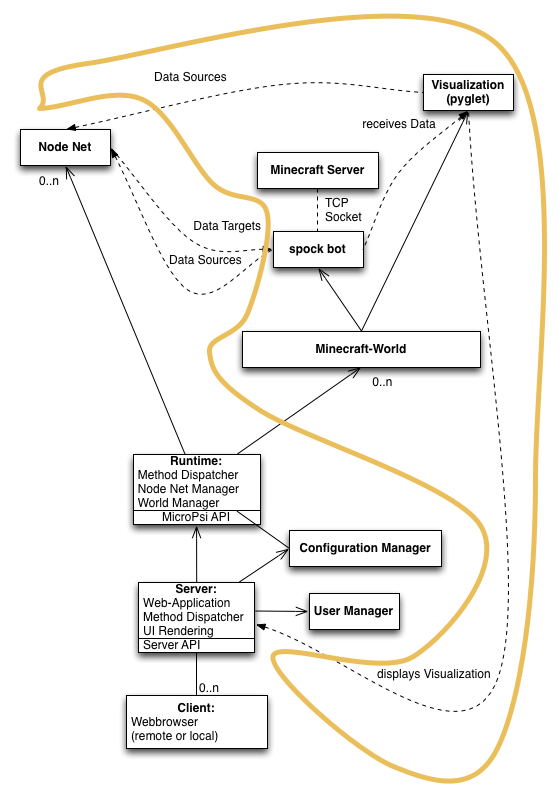
\includegraphics[width=10cm]{graphics/UML_MicroPsi_mit_spock_und_rahmen}
  \caption{The new architecture of MicroPsi with the Minecraft interface. New modules are framed orange.}
  \label{uml_mc}
\end{figure}

... graphic/UML of the project as a whole ...
... illustration of the event loop ...

% TODO je nach Größe des Kapitels, das hier vielleicht eine Ebene höher ziehen (versuche dich hier erstmal nur auf die fertige Lösung zu konzentrieren und warum du dich dafür entschieden hast. Es ist nicht interessant, was du sonst alles ausprobiert hast, außer dass du konkret angibst, warum du dich für die jetztige Implementierung im Vergleich zu anderen entschieden hast)

\section{A! Case Study}

The functionality is to be tested with a simple Braitenberg-vehicle experiment.

\subsection{Experiment}
... experiment to test functionality of the system ...
... scope: only a simple test for time reasons ...

\subsubsection{Braitenberg Vehicle}
... simplest proof of concept of a microPsi agent ...